\documentclass[a4paper,10pt]{article}

\usepackage[utf8]{inputenc}
\usepackage[left=0.5in,right=0.5in,top=1in,bottom=1in]{geometry}
\usepackage{amsmath,amssymb,amsfonts}
\usepackage{pgfplots,graphicx,calc,changepage,caption}
\pgfplotsset{compat=newest}
\usepackage{enumitem}
\usepackage{fancyhdr}
\usepackage[colorlinks = true, linkcolor = blue]{hyperref}

% Syntax highlighting
\usepackage{listings}
\usepackage{xcolor}

\definecolor{codegreen}{rgb}{0.40,0.62,0.07}
\definecolor{codegray}{rgb}{0.5,0.5,0.5}
\definecolor{codeblue}{rgb}{0.09,0.57,0.73}
\definecolor{backcolour}{rgb}{1,1,1}

\lstdefinestyle{mystyle}{
    backgroundcolor=\color{backcolour},   
    commentstyle=\color{codegreen},
    keywordstyle=\color{magenta},
    numberstyle=\tiny\color{codegray},
    stringstyle=\color{codeblue},
    basicstyle=\ttfamily\small,
    breaklines=true,                     
    keepspaces=true,                 
    numbers=left,                    
    numbersep=5pt,                  
    showspaces=false,
    showstringspaces=false,
    showtabs=false,                  
    tabsize=4
}

\lstset{style=mystyle}

\newcommand{\nats}{\mathbb{N}}
\newcommand{\reals}{\mathbb{R}}
\newcommand{\rats}{\mathbb{Q}}
\newcommand{\ints}{\mathbb{Z}}
\newcommand{\pols}{\mathcal{P}}
\newcommand{\cants}{\Delta\!\!\!\!\Delta}
\newcommand{\eps}{\varepsilon}
\newcommand{\st}{\backepsilon}
\newcommand{\abs}[1]{\left| #1 \right|}
\newcommand{\dom}[1]{\mathrm{dom}\left(#1\right)}
\newcommand{\for}{\text{ for }}
\newcommand{\dd}[1]{\mathrm{d}#1}
\newcommand{\spn}{\mathrm{sp}}
\newcommand{\nul}{\mathcal{N}}
\newcommand{\col}{\mathrm{col}}
\newcommand{\rank}{\mathrm{rank}}
\newcommand{\norm}[1]{\lVert #1 \rVert}
\newcommand{\inner}[1]{\left\langle #1 \right\rangle}
\newcommand{\pmat}[1]{\begin{pmatrix} #1 \end{pmatrix}}
\renewcommand{\and}{\text{ and }}

\newsavebox{\qed}
\newenvironment{proof}[2][$\square$]
    {\setlength{\parskip}{0pt}\par\textit{Proof:} #2\setlength{\parskip}{0.25cm}
        \savebox{\qed}{#1}
        \begin{adjustwidth}{\widthof{Proof:}}{}
    }
    {
        \hfill\usebox{\qed}\end{adjustwidth}
    }

\pagestyle{fancy}
\fancyhead{}
\lhead{Caleb Jacobs}
\chead{APPM 5600: Numerical Analysis I}
\rhead{Homework \#1}
\cfoot{}
\setlength{\headheight}{35pt}
\setlength{\parskip}{0.25cm}
\setlength{\parindent}{0pt}

\captionsetup{width = 0.5\textwidth}

\begin{document}
\begin{enumerate}[label = \arabic*.)]
    \item How would you perform the following calculations to avoid cancellation?
        \begin{enumerate}[label = \roman*.]
            \item Evaluate $\sqrt{x + 1} - 1$ for $x \simeq 0$.
            
            First, let's rewrite our expression as
            \[
                (\sqrt{x + 1} - 1) \cdot \frac{\sqrt{x + 1} + 1}{\sqrt{x + 1} + 1} = \frac{x}{\sqrt{x + 1} + 1}.
            \]
            Using this new expression to compute $\sqrt{x + 1} - 1$ is favorable because it avoids cancellation error for $x \simeq 0$ by removing the similar term subtraction in the numerator and replaces it with safe addition in the denominator.
            
            \item Evaluate $\sin(x) - \sin(y)$ for $x \simeq y$.
            
            Using a trig identity, we can rewrite our expression as
            \[
                \sin(x) - \sin(y) = 2 \sin\left(\frac{x - y}{2}\right) \cos\left( \frac{x + y}{2} \right).
            \]
            
            Although it looks like we haven't done much to remove the subtraction, we have mitigated the cancellation and rounding error associated with the subtraction. When we use $ \sin(x) - \sin(y) $ we are subtracting two numbers that are already approximated in the computer (i.e. the computer introduced some extra error in computing sin of our floating point numbers). Subtracting the two 
            
            \item Evaluate $\frac{1 - \cos(x)}{\sin(x)}$ for $x \simeq 0$.
            
            We can rewrite the expression above using a conjugate and a trig identity as follow:
            \begin{align*}
                \frac{1 - \cos(x)}{\sin(x)} \cdot \frac{1 + \cos(x)}{1 + \cos(x)} &= \frac{1 - \cos^2(x)}{\sin(x) (1 + \cos(x))} \\
                &= \frac{\sin^2(x)}{\sin(x) (1 + \cos(x))} \\
                &= \frac{\sin(x)}{1 + \cos(x)}.
            \end{align*}
            The rewritten expression no longer contains the cancellation in the numerator introduced by the $1 - \cos(x)$ for $x \simeq 0$ and instead has a simple and accurate $\sin(x)$ in the numerator. In the denominator, our new expression has an accurate addition that will not shoot to 0 when $x \simeq 0$.
            
        \end{enumerate}
    
    \newpage
    \item Consider the polynomial
        \[
            p(x) = (x - 2)^9  = x^9 - 18x^8 + 144x^7 - 672x^6 + 2016x^5 - 4032x^4 + 5376x^3 - 4608x^2 + 2304x - 512.
        \]
        \begin{enumerate}[label = \roman*.]
            \item Plot $p(x)$ for $x = 1.920, 1.921, 1.922, \ldots, 2.080$ (i.e. $x = [1.920 : 0.001 : 2.080]$) evaluating $p$ via its coefficients.
            
            \begin{figure}[h!]
                \centering
                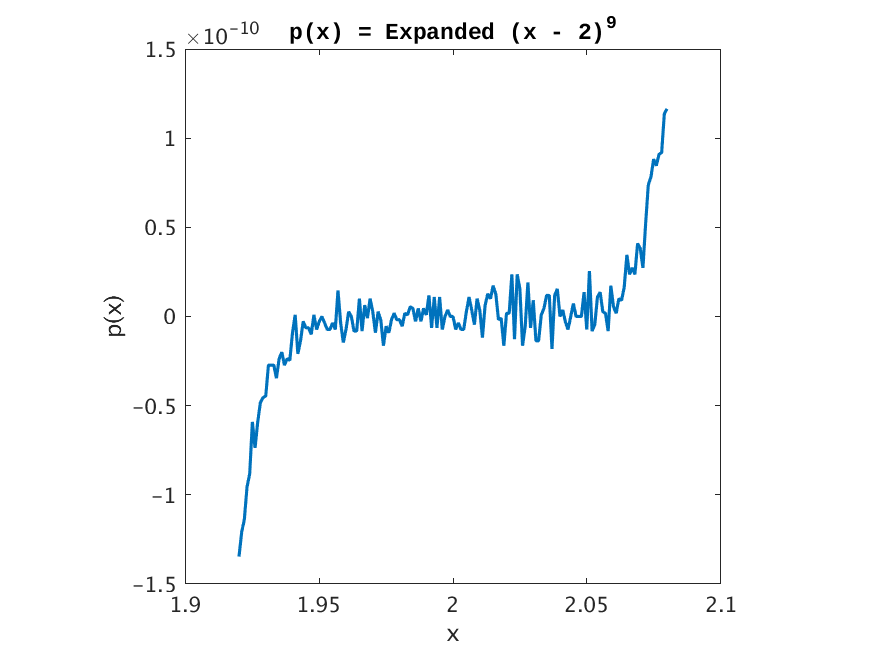
\includegraphics[width = 0.5\textwidth]{images/2.i.png}
                \label{fig:2.i}
            \end{figure}
            
            \item Produce the same plot again, now evaluating $p$ via the expression $(x - 2)^9$.
            
            \begin{figure}[h!]
                \centering
                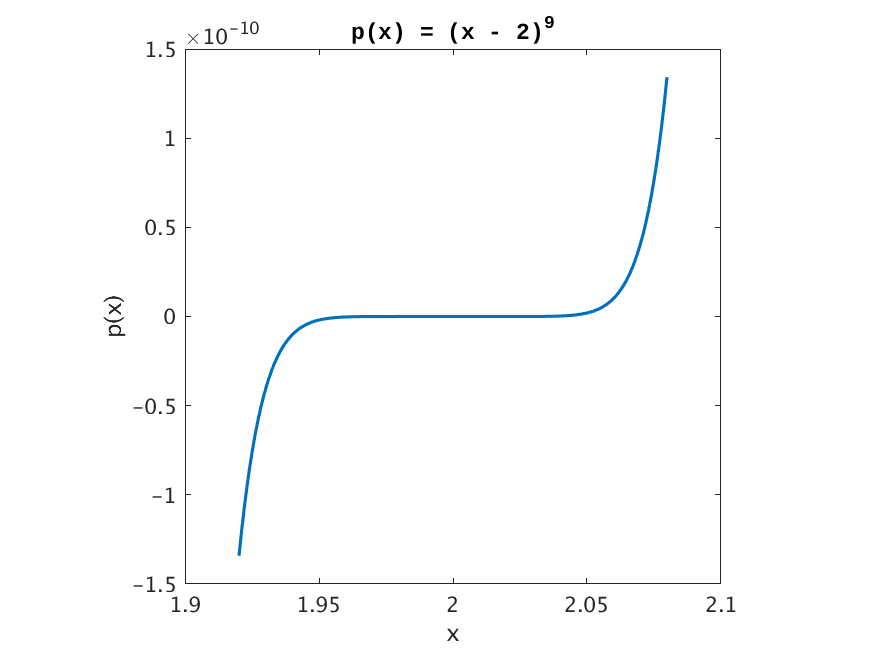
\includegraphics[width = 0.5\textwidth]{images/2.ii.png}
                \label{fig:2.ii}
            \end{figure}
            
            \item What is the difference? What is causing the discrepancy? Which plot is correct?
            
            The plot in part i is considerably more noisy than the plot in part ii. The difference in the results are due to the extra cancellation and rounding error caused by the abundance of addition and subtraction of small magnitude numbers with relatively large magnitude numbers. The plot in part ii is the more correct plot because it doesn't suffer from the increased error imposed by the expanded polynomial coefficients. 
        \end{enumerate}
        
        \newpage
        \item \textbf{Cancellation of terms.} Consider computing $y = x_1 - x_2$ with $\Tilde{x}_1 = x_1 + \Delta x_1$ and $\Tilde{x}_2 = x_2 + \Delta x_2$ being approximations to the exact values. If the operation $x_1 - x_2$ is carried out exactly we have $\Tilde{y} = y + \underbrace{(\Delta x_1 - \Delta x_2)}_{\Delta y}$.
        
            \begin{enumerate}[label = \roman*.]
                \item Find upper bounds on the absolute error $\abs{\Delta y}$ and the relative error $\abs{\Delta y} / \abs{y}$, when is the relative error large?
                
                \textbf{Absolute error upper bound:}
                \begin{align*}
                    \abs{\Delta y} &= \abs{\Delta x_1 - \Delta x_2} \\
                    &< \abs{\Delta x_1} + \abs{\Delta x_2}.
                \end{align*}
                
                \textbf{Relative error upper bound:} Using our absolute error upper bound, we have
                \begin{align*}
                    \frac{\abs{\Delta y}}{y} &< \frac{\abs{\Delta x_1} + \abs{\Delta x_2}}{\abs{y}} \\
                    &= \frac{\abs{\Delta x_1} + \abs{\Delta x_2}}{\abs{x_1 - x_2}}
                \end{align*}
                
                \item First manipulate $\cos(x + \delta) - \cos(x)$ into an expression without subtraction. Then, plot the difference between your expression and $\cos(x + \delta) - \cos(x)$ for $\delta = 10^{-16}, 10^{-15}, \ldots, 10^{0}$.
                
                We can remove subtraction from the expression above by rewriting it as
                \begin{align*}
                    \cos(x + \delta) - \cos(x) &= -2\sin\left(\frac{x + \delta + x}{2}\right)\sin\left(\frac{x + \delta - x}{2}\right) \\
                    &= -2\sin\left(\frac{2x + \delta}{2}\right) \sin\left(\frac{\delta}{2}\right)
                \end{align*}
                
                With our rewritten expression, we can generate the difference plot below:
                \begin{figure*}[h!]
                    \centering
                    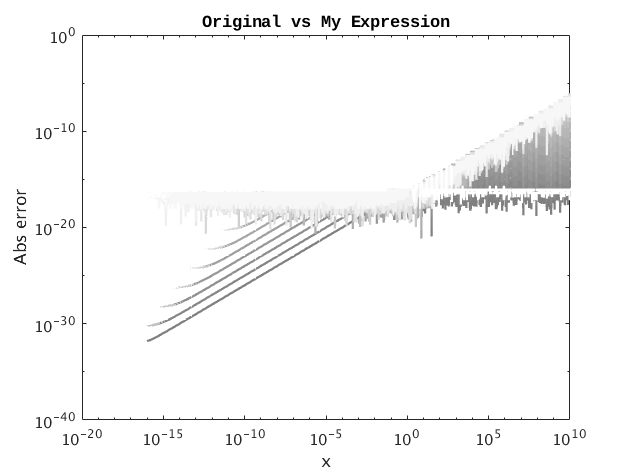
\includegraphics[width=0.5\textwidth]{images/3.iii.png}
                    \caption{Absolute error between the original difference function and my expression. Darker lines = smaller values of $ \delta $ starting at $ \delta = 10^{-16} $ up to $ \delta = 1 $ for the whitest line.}
                \end{figure*}
                
                \item Taylor expansion yields $f(x + \delta) - f(x) = \delta f'(x) + \frac{\delta^2}{2!}f''(\xi), \xi \in [x, x+\delta].$ Use this expression to approximate $\cos(x + \delta) - \cos(x)$  for the same values of $\delta$ as in (ii). For what values of $\delta$ is each method better?
                
                For really small values of $ \delta $, the Taylor expansion is the most accurate but my expression is also very accurate. The accuracy of the Taylor expansion when $ \delta $ is small makes sense because Taylor expansions are most accurate near their expansion center. As $ \delta $ gets closer to 1, the original expression and my expression both perform accurately with little difference in there calculations. The Taylor expansion does not perform well for $ \delta $ close to 1 because we don't have enough terms to extend the accuracy that far from the center. With that being said, my expression has the most reliable computations of the three expressions.
                
              \begin{figure*}[h!]
                  \centering
                  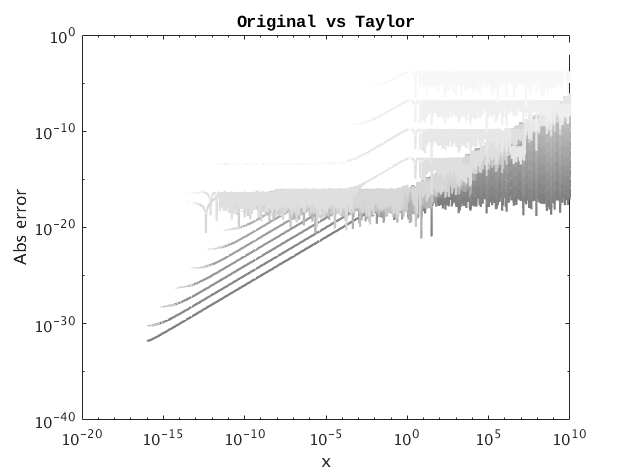
\includegraphics[width=0.45\textwidth]{images/3.i.png}
                  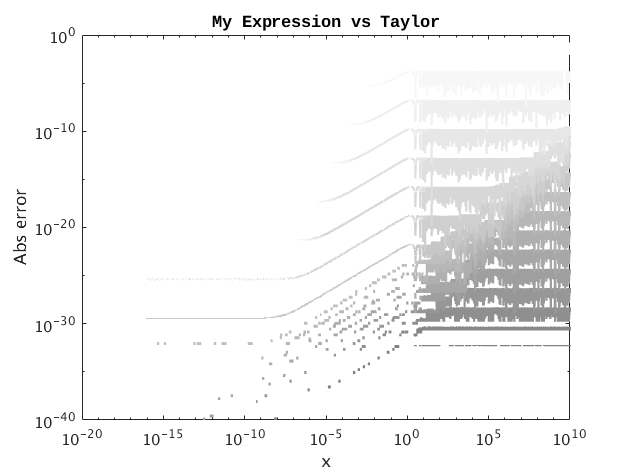
\includegraphics[width=0.45\textwidth]{images/3.ii.png}
              \end{figure*}  
            \end{enumerate}
            
            \item Show that $(1 + x)^n = 1 + nx + o(x)$ as $x \to 0$ where $n \in \ints$.
             
             Consider 
             \begin{align*}
                \lim_{x \to 0} \frac{(1 + x)^n - (1 + nx)}{x} &= \lim_{x \to 0}  \left(\frac{(1 + x)^n - 1)}{x} - n\right) \\
                &= \lim_{x \to 0}  \left(\frac{(1 + x)^n - 1)}{x}\right) - \lim_{x \to 0}n \\
                &= \lim_{x \to 0}  \left(\frac{(1 + x)^n - 1)}{x}\right) - n \\
                &= \lim_{x \to 0}  \left(\frac{n(1 + x)^{n-1})}{1}\right) - n \\
                &= n - n = 0.
             \end{align*}
            Therefore
            \[
                (1 + x)^n - (1 + nx) = o(n)
            \]
            or in other words
            \[
                (1 + x)^n = 1 + nx + o(n).
            \]
            
            \item Show that $ x \sin (\sqrt{x}) = O(x^{3/2}) $ as $x \to 0^+$.
            
            Suppose we have any $ \varepsilon > 0 $ and $ x \in [0, \varepsilon) $. Then
            \[
                \abs{\frac{x \sin(x) \sqrt{x}}{x^{3/2}}} = \abs{\frac{x^{3/2} \sin(x)}{x^{3/2}}} = \abs{\sin(x)} \leq 1 = M.
            \]
            Therefore, $ x \sin (\sqrt{x}) = O(x^{3/2}) $ as $ x \to 0^+ $.
            
            \item The function $f(x) = (x - 5)^9$ has a root at $x = 5$ and is monotonically increasing (decreasing) for $x > 5$ $(x < 5)$ and should thus be a suitable candidate for your function above. Set $a = 4.8$ and $b = 5.3$ and $tol = 1e-4$ and use bisection with:
                \begin{enumerate}[label = \roman*.]
                    \item $f(x) = (x - 5)^9$.
                    
                    Using my bisection code converges in 13 iterations to a root of $ x = 5.0000280761718763 $.
                    
                    \item The expanded version of $(x - 5)^9$.
                    
                    Using my bisection code on the expanded  polynomial converges in 13 iterations to a root of $ x = 5.1221740722656248 $.
                    
                    \item Explain what is happening.
                    
                    From question 2, we can see that a fully expanded polynomial may not always be the best idea when using floating point numbers. The loss of accuracy when using the bisection method in part (ii) can be attributed to the expanded polynomial. The expanded polynomial adds and subtracts relatively large and relatively small numbers which causes cancellation and rounding error to run rampant causing loss in significant digits. Thus the best accuracy we can hope for in the expanded polynomial is much less than the compact polynomial.
                \end{enumerate} 
\end{enumerate}

\newpage
\rule{\textwidth}{0.4pt}
\lstinputlisting[language = matlab]{bisection.m}
\rule{\textwidth}{0.4pt}
\end{document}